\section{Hardware}
This section is dedicated to show all the electronic components we chose and how they work together. As described earlier the PCB containing all the components will be manufactured by Seeedstudio. They manufacture PCBs with other hardware components and they sell quite a number of different breakout boards and other developpement parts. A request made by CHIC managing team was to source as many components as possible at Seeedstudio. Of course not all components we needed were available by them so some of the components are from different sources.

Hardware :
\begin{itemize}
\item{Beaglebone black, will be further mentioned as BBB}
\item{SD card (containing the Operating System)}
\item{PCB}
\item{Wl1835mod WIFI and bluetooth module}
\item{Capacitive touch screen}
\item{ADXL-345 accelerometer}
\item{Some other tension regulators and a battery drive}
\end{itemize}

\subsection{Beaglebone Black}
The BBB is an open-hardware microcomputer very famous for development. It uses an ARM processor from Texas Instruments, the AM335X. It is clocked at 1GHz.
\begin{itemize}
  \item{ AM335x 1GHz ARM® Cortex-A8 }
  \item{512MB DDR3 RAM}
  \item{4GB 8-bit eMMC on-board flash storage}
  \item{Ethernet}
  \item{2x 46 pin headers}
  \item{Open source}
  \item{...}
\end{itemize}



% \begin{table}[!htbp]
%   \begin{center}
%     \begin{tabular}{|l|r|r|}%p{5cm}|}
%       \hline
%         measurement N$^{\circ}$ & CW [mNm] & CCW [mNm]\\ \hline %\hline
%         test two & 2.24e-4 & -6.32e-4 \\ \hline
%         2 & 2.073-4 & -6.39e-4\\ \hline
%         3 & 2.72e-4 & -6.64e-4\\ \hline
%         4 & 2.46e-4 & -6.46e-4\\ \hline
%         5 & 2.72e.4 & -6.64e-4\\ \hline \hline
%         mean & 2.44e-4 & -6.49e-4\\
%          \hline
%     \end{tabular}
%   \end{center}
%   \caption {Main BBB specifications} \label{tab:bbb specs}
% \end{table}

\subsection{Screen and Touchscreen}
At the current state of our prototype the main function is to view images and text. Therefor a good screen we realistic colors is necessary to have a good user experience.
We first ordered a resistive touchscreen BBB cape (4DCAPE-70T 4D systems) available from seeedstudio to see how its was made and to see if the resistive technology was applicable to our project. We quickly realised that the resistive tuchscreen was not very adapted to manipulate photos. Especially the very well known “swipe” geasture to move from one photo to another was impossible to do with the resistive touchscreen.
This screens colors were coded on 16 bits and the viewing angle was quite bad.
So we looked for a similar screen but one using a capacitive touchscreen and with more colors. We started by looking on chinese sites which had the cheapest screens of course. But the cheap chinese screens were lacking documentation. At the time we were unfamiliar with the interface the screens used and we needed at least a datasheet to get going.
 Finally we chose a screen we found on Mouser which had good documentation and especially there was an existing driver for the touchscreen IC in the linux kernel we were going to use.
 The screen is actually a package containing the screen and its driver, the touch-screen and its driver and the backlight LED array. This package can be seen in fig.
 \begin{figure}[!htb]
     \centering
     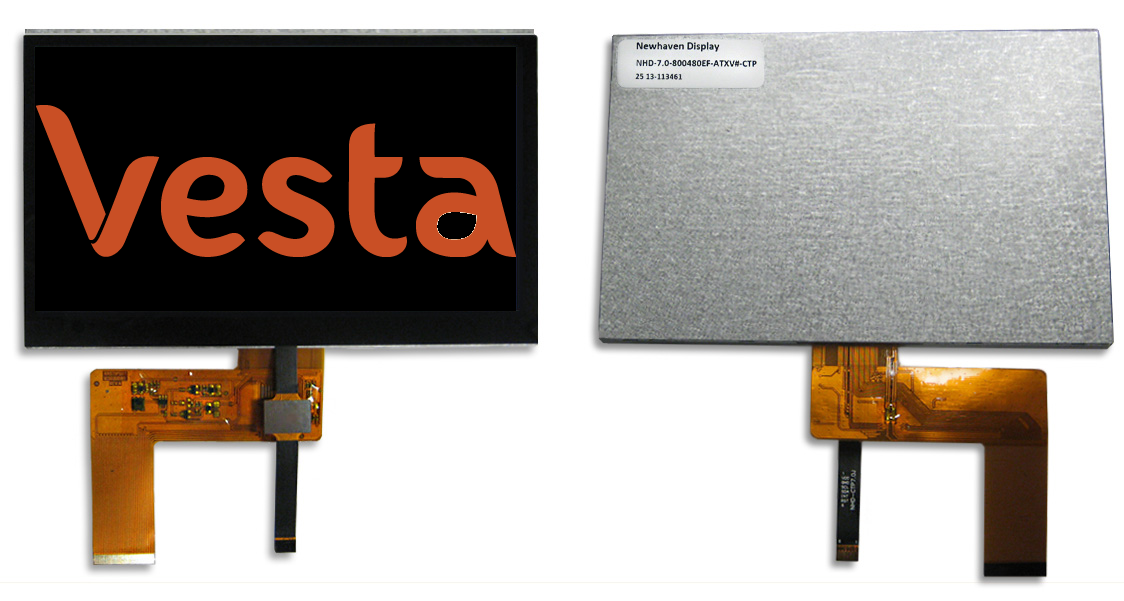
\includegraphics[width=0.5\textwidth,keepaspectratio]{chap/hardfig/newhaven_screen_image}
     \caption{Screen package.}
     \label{fig:screen package}
 \end{figure}

 Individual components are discribed in the following sub chapters.

\subsubsection{Screen}
The screen is the NHD-7.0-800480EF-ATXV\#-CTP from Newhaven Display. The specifications of the screens are listed bellow.
\begin{itemize}
  \item {7" Diagonal}
  \item{Resolution: 800xRGBx480}
  \item{24 bit digital RGB interface}
  \item{White led backlight}
  \item{55-65$^{\circ}$ Top-bottom viewing angle }
  \item{70 $^{\circ}$ left-rigth viewing angle}
  \item{}
\end{itemize}


\subsubsection{Touchscreen}
\begin{itemize}
  \item {Capacitive touch panel with built-in Focaltech ft5x06 controller}
  \item {i2c interface}
  \item {linux kernel compatible}
\end{itemize}
The touchpanel is very smooth and reactive. The
\subsubsection{Backlight}
The backlight is a quite bright white led array consisting of 5x3 LEDs. the configuration can be seen in fig.\ref{fig:backlight_led}

\begin{figure}[!htb]
    \centering
    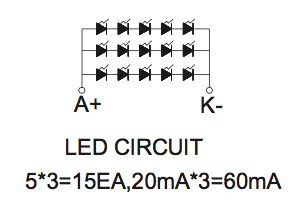
\includegraphics[width=0.5\textwidth,keepaspectratio]{chap/hardfig/backlight_led_circuit}
    \caption{Backlight LED array configuration.}
    \label{fig:backlight_led}
\end{figure}

This LED array requires 60 mA at 16 V to operate. This power is taken directly from the 3.3v of the BBB and boosted to the required voltage by FAN5333A LED driver from Fairchild semiconductors.
This IC is a general purpose LED driver which can be controller with a PWM imput.
Our implementation of the FAN5333A is pictured in fig.

% \begin{figure}[!htb]
%     \centering
%     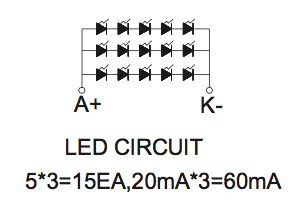
\includegraphics[width=0.5\textwidth,keepaspectratio]{chap/hardfig/backlight_led_circuit}
%     \caption{FAN5333A Backlight LED driver implementation.}
%     \label{fig:backlight driver schematics}
% \end{figure}

\subsection{Wireless Communication}
\subsubsection{Wlan}
\subsubsection{Bluetooth}
\subsubsection{Power management}
\subsection{Front LED}
The LED is there to inform the user of a new message. Therefor it could be quite low power. Seeedstudio only had an RGB LED which we ordered although for the final led we will use is a warm white single color LED.

We want it to flash in a heartbeat patern. This is achieved by using a PWM pin of the BBB
\subsection{Power management}
\subsection{Batteries and charger}
\subsection{PCB}
\subsection{Cost estimates}
